\documentclass[11pt]{article}
\usepackage[margin=1in]{geometry}
\usepackage{amsmath,amssymb,amsthm,bm,booktabs,graphicx,hyperref}
\usepackage[numbers,sort&compress]{natbib}
\setlength{\emergencystretch}{2em}

\newtheorem{definition}{Definition}
\newtheorem{proposition}{Proposition}
\newtheorem{conjecture}{Conjecture}
\newcommand{\MI}{\operatorname{I}}
\newcommand{\Hspace}{\mathcal H}

\title{The Observer World-Tube Principle:\\
A Variational Extension of the Quantum Factorization Problem}
\author{Mahsa Keikha, PhD}
\date{Working paper, version 0.1}

\begin{document}
\maketitle

\begin{abstract}
Tegmark proposed that observer-like physical systems may be distinguished by
information, integration, independence, and nontrivial dynamics, and connected
these properties to the problem of selecting a preferred tensor factorization
of Hilbert space. A fixed factorization, however, identifies an observer with a
fixed collection of degrees of freedom. Biological and computational identity
can persist while physical components and internal representations change. We
therefore propose that the relevant mathematical object is not a factorization
but a trajectory through factorization space, called an observer world-tube.
We introduce an exact Gaussian baseline that combines directed internal
integration, conditional environmental insulation, and predictive persistence.
We prove that the directed term rejects contemporaneously correlated but
dynamically uncoupled systems, a failure mode of static mutual information. We
then formulate a regularized action for time-dependent subsystem boundaries and
recover a planted moving module in an initial numerical experiment. The score is
not presented as a measure of phenomenal consciousness. It is a falsifiable
candidate principle for selecting persistent observer-like organization, and a
route toward a gauge-invariant quantum formulation.
\end{abstract}

\section{Motivation}

Tegmark's perceptronium program asks which physical properties distinguish
observer-like matter and whether those properties can help select the spatial
factorization perceived by observers \citep{tegmark2015}. The program exposes a
tension. Independence favors a weak interaction Hamiltonian, but maximizing it
alone selects dynamically trivial structures. Conscious organization, if it is
physical, must be sufficiently insulated to have its own dynamics and
sufficiently coupled internally to change as a whole.

Existing work already supplies temporal and causal measures of integration
\citep{oizumi2016,mediano2025} and transformation-invariant measures of
dynamical independence \citep{barnett2023}. Our proposal is therefore not merely
to add a temporal mutual information term. We instead let the factorization
itself change. This shifts the object of study from an instantaneous subsystem
to a persistent path in a space of possible subsystems.

\section{Exact Gaussian baseline}

Let
\begin{equation}
X_{t+1}=AX_t+\epsilon_t,\qquad
\epsilon_t\sim\mathcal N(0,Q),\qquad \rho(A)<1.
\end{equation}
The stationary covariance $\Sigma$ uniquely solves
\begin{equation}
\Sigma=A\Sigma A^{\mathsf T}+Q.
\end{equation}
All information quantities below are therefore analytic functions of $A$ and
$Q$.

For candidate subsystem $S$ and bipartition $S=U\sqcup V$, define
\begin{equation}
J_\tau(U,V)=
\MI(X_U^{t+\tau};X_V^t\mid X_U^t)
+\MI(X_V^{t+\tau};X_U^t\mid X_V^t).
\end{equation}

\begin{definition}[Directed integration]
\begin{equation}
\mathcal J_\tau(S)=\frac{1}{|S|}
\min_{U\sqcup V=S}J_\tau(U,V).
\end{equation}
\end{definition}

The normalization is provisional and will be included in the ablation study.
The minimum implements a weakest-link requirement. Unlike simultaneous mutual
information, each cross-prediction conditions on the target part's own present.

\begin{definition}[Environmental leakage]
\begin{equation}
\mathcal L_\tau(S)=\frac{1}{|S|}
\MI(X_S^{t+\tau};X_{\bar S}^{t}\mid X_S^t).
\end{equation}
\end{definition}

Let $P_\tau(S)$ be the mean squared canonical correlation between $X_S^t$ and
$X_S^{t+\tau}$. We define bounded factors
\begin{equation}
G_\tau=1-2^{-\mathcal J_\tau},\qquad
K_\tau=2^{-\mathcal L_\tau},
\end{equation}
and a baseline score
\begin{equation}
\Omega_\tau(S)=\left(G_\tau K_\tau P_\tau\right)^{1/3}.
\end{equation}
The geometric mean makes all three properties necessary. Other aggregations
must be compared rather than assumed.

\begin{proposition}[Rejection of static common correlation]
Suppose $A$ is diagonal and the innovations are independent across time, while
$Q$ may contain arbitrary contemporaneous cross-correlations. Then for every
bipartition and every positive lag, $J_\tau(U,V)=0$.
\end{proposition}

\begin{proof}
For diagonal $A$, $X_U^{t+\tau}$ is a function of $X_U^t$ and innovations after
time $t$. Those innovations are independent of $X_V^t$. Hence
$X_U^{t+\tau}\perp X_V^t\mid X_U^t$, so the first conditional mutual
information vanishes. Interchanging $U$ and $V$ proves the second term also
vanishes.
\end{proof}

This proposition does not solve causal identification in the presence of hidden
variables. It establishes a narrower and useful guarantee: simultaneous
correlation alone is insufficient.

\section{Observer world-tubes}

Let $\mathfrak F_{d,n}$ be a space of factorizations
$\Hspace\cong\Hspace_S\otimes\Hspace_E$ with dimensions $d$ and $n/d$.
An observer candidate is a curve
\begin{equation}
\gamma:t\longmapsto F_t\in\mathfrak F_{d,n}.
\end{equation}
In a finite classical system, its discrete analog is a sequence
$S_0,S_1,\ldots,S_T$. Its support in index-time space is
\begin{equation}
\mathcal W=\{(i,t):i\in S_t\},
\end{equation}
which we call an observer world-tube.

We propose the action
\begin{align}
\mathcal A(\mathcal W)
=&\sum_t\left[
\alpha\mathcal J_\tau(S_t,S_{t+\tau})
-\beta\mathcal L_\tau(S_t,S_{t+\tau})
+\chi\mathcal P_\tau(S_t,S_{t+\tau})
\right]\\
&-\lambda\sum_t d_{\mathfrak F}(S_t,S_{t+1}).
\end{align}
The transport term $\mathcal P$ rewards continuity of organization. The metric
term penalizes arbitrary changes of factorization without requiring unchanging
material membership.

For the quantum theory, tensor factorizations can be represented by unitary
transformations modulo local basis changes. Schematically,
\begin{equation}
\mathfrak F_{d,n}\simeq
U(n)/\left(U(d)\otimes U(n/d)\right),
\end{equation}
subject to the correct stabilizer and discrete identifications. If $U_t$
represents the factorization path, the horizontal part of
$U_t^\dagger\dot U_t$ measures genuine factorization drift, while the vertical
part is a local relabeling. This is the point at which a gauge connection enters
naturally.

\begin{conjecture}[Observer world-tube principle]
For physical systems containing a dynamically integrated and conditionally
insulated process, a gauge-invariant version of $\mathcal A$ has a stable local
maximum whose world-tube follows organizational identity through changes in
physical realization.
\end{conjecture}

\section{Initial numerical experiment}

We constructed a seven-node Gaussian system with a planted three-node coherent
module. At each of five time steps, one node leaves and another enters. The
implemented dynamic program evaluates all $\binom{7}{3}=35$ candidate boundaries
at every step, combines the fixed-boundary baseline with directed transport and
a boundary-motion cost, and exactly recovers the planted sequence
\begin{equation}
(0,1,2)\to(1,2,3)\to(2,3,4)\to(3,4,5)\to(4,5,6).
\end{equation}

\begin{figure}[ht]
\centering
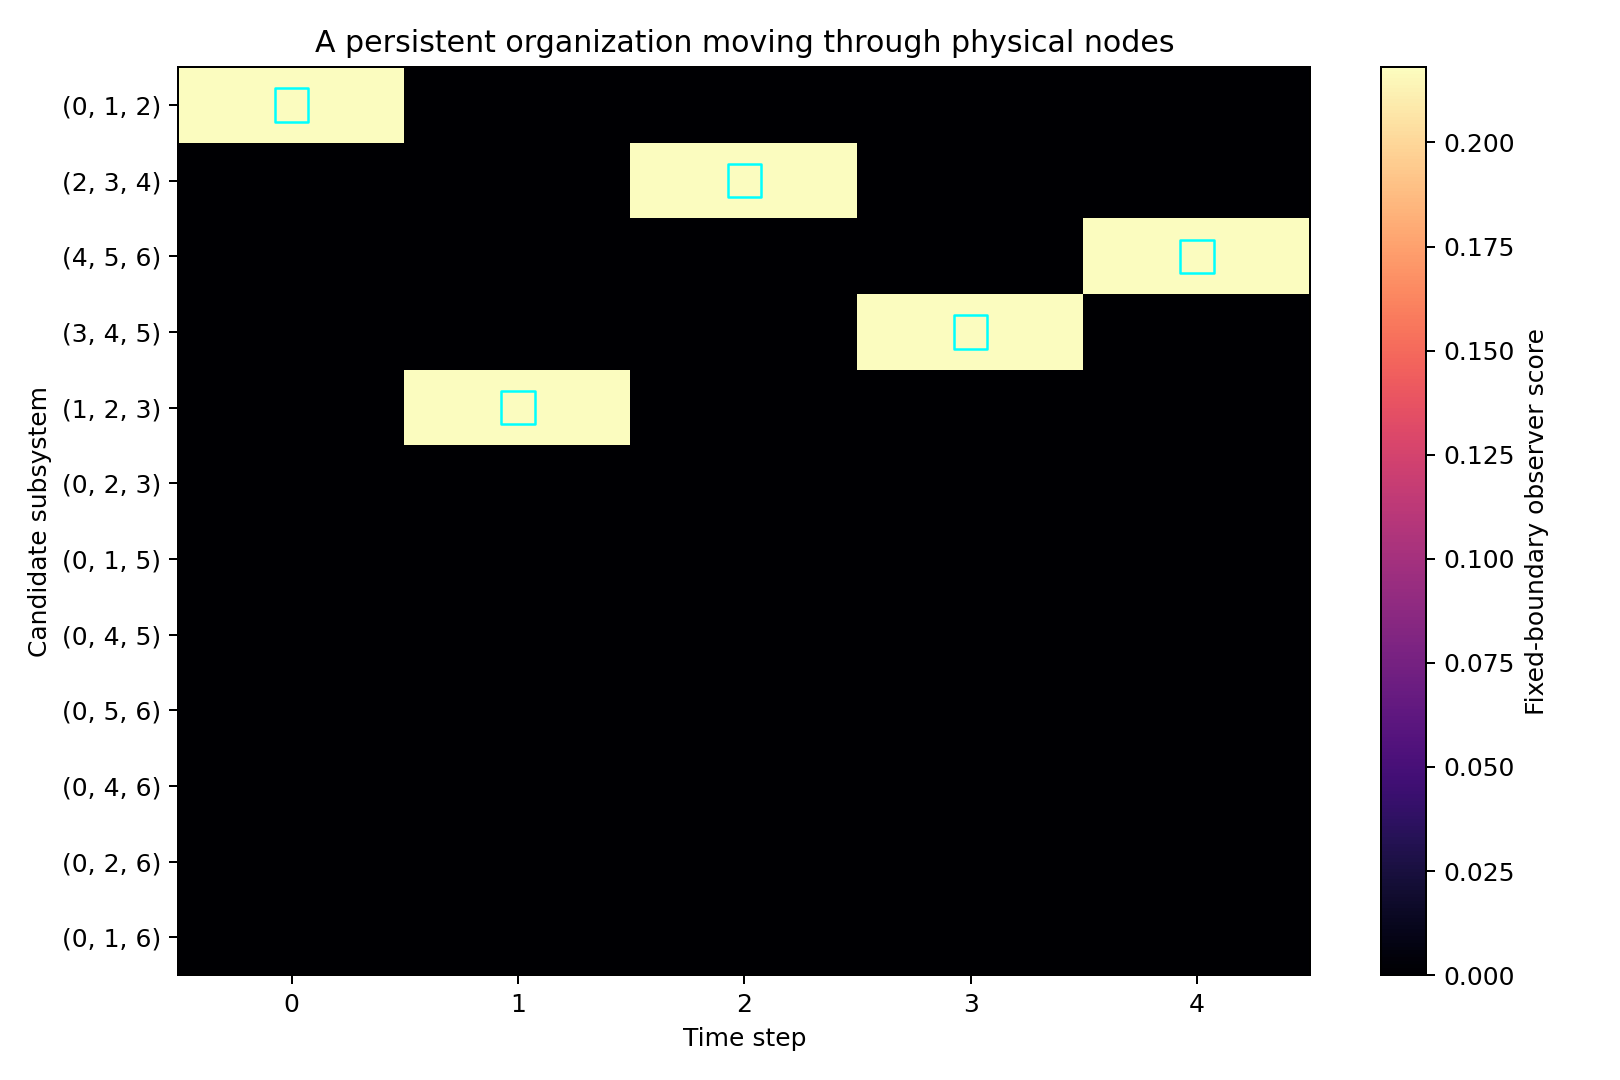
\includegraphics[width=0.92\linewidth]{../docs/worldtube_baseline.png}
\caption{Fixed-boundary scores across time. Cyan squares mark the world-tube
selected by the path action. This is a proof-of-concept recovery experiment,
not evidence about biological consciousness.}
\end{figure}

\section{Falsification program}

The proposal should be rejected or revised if any of the following persist
under preregistered tests: the path is unstable under small coordinate changes;
null systems produce equally stable world-tubes; fixed-factorization baselines
perform equally well on moving-identity tasks; or the quantum action retains the
same dynamically trivial optimum that motivated the extension.

The next mathematical tasks are to prove invariance properties, derive recovery
bounds for planted moving modules, formalize the quotient geometry, and compare
the action against geometric integrated information, $\Phi$ID, dynamical
independence, causal emergence, and dynamic community detection.

\section{Interpretation}

The intended synthesis can be stated compactly. Space corresponds to a
factorization that localizes interaction. Time is the ordering along which
predictive structure changes. An observer is not a point in either space, but a
persistent integrated path through both. The mathematics developed here does
not explain subjective experience. It proposes a sharper physical question:
which evolving boundary makes a system most capable of being a process in its
own right?

\bibliographystyle{plainnat}
\bibliography{references}
\end{document}
